\section{Subsystems}

\subsection{Use-Case Diagrams}

\subsubsection{"Invite Only" Application}
The "Invite Only" application serves as the means through which any user will interact with the "Invite Only" system. The application will run on multiple mobile operating systems and its specific use cases are depicted in figure \ref{fig:invite_only_use_case}.

\subsubsection{User Library}
The User Library provides the interface through which the system will user's are authenticated and their details stored. This includes the management of identification documents linked to users. See figure \ref{fig:user_library_use_case} for the specific use cases of this service.

\subsubsection{Space Library}
The Space Library provides an interface for the management of access-controlled spaces. This includes the creation, updating and deletion of these spaces and their details. Figure \ref{fig:space_library_use_case} shows the use cases of this service in more detail.

\subsubsection{Access Library}
The Access Library is responsible for allowing or denying access to an access-controlled space. It will also record who entered or left a space and at what times. The use case diagram shown in figure \ref{fig:access_library_use_case} further details how this service works.

\subsubsection{Invite Library}
The Invite Library provides an interface through which invite codes can be generated and validated. The validation of an invite code leads to access being granted to an access-controlled space. See figure \ref{fig:invite_library_use_case} for the use cases of the Invite Library.

\begin{figure}[H]
  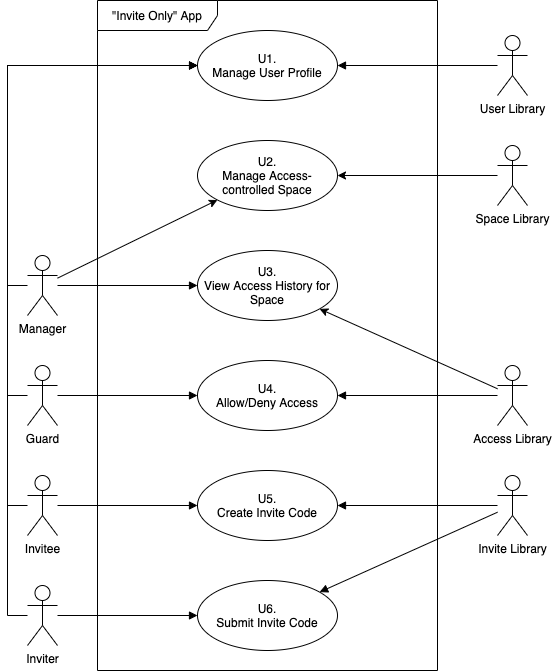
\includegraphics[width=1.0\textwidth]{documentation/software_requirements_specification/subsystems/invite_only_use_case.png}
  \caption{"Invite Only" Application Use Case Diagram}
  \label{fig:invite_only_use_case}
\end{figure}

\begin{figure}[H]
  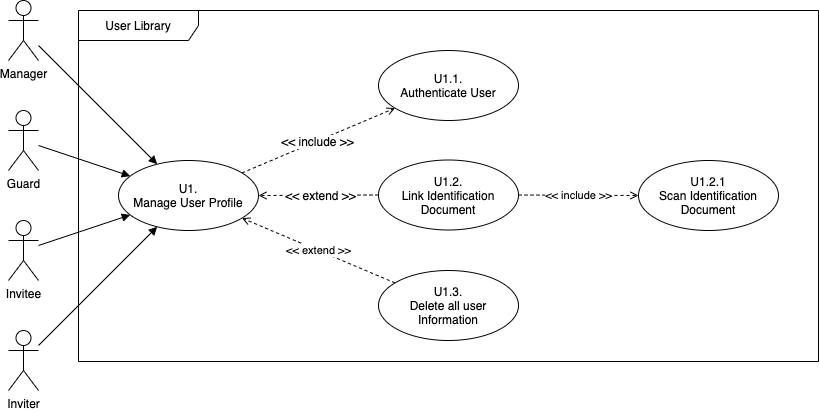
\includegraphics[width=1.0\textwidth]{documentation/software_requirements_specification/subsystems/user_library_use_case.png}
  \caption{User Library Use Case Diagram}
  \label{fig:user_library_use_case}
\end{figure}

\begin{figure}[H]
  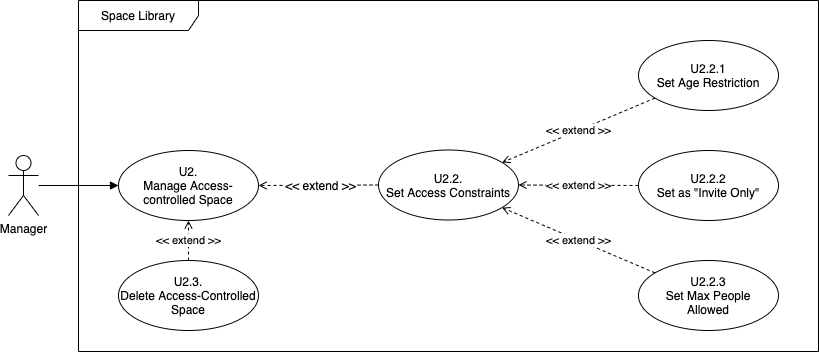
\includegraphics[width=1.0\textwidth]{documentation/software_requirements_specification/subsystems/space_library_use_case.png}
  \caption{Space Library Use Case Diagram}
  \label{fig:space_library_use_case}
\end{figure}

\begin{figure}[H]
  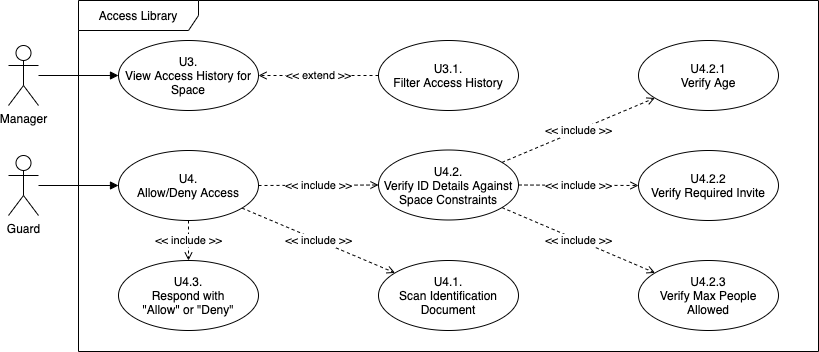
\includegraphics[width=1.0\textwidth]{documentation/software_requirements_specification/subsystems/access_library_use_case.png}
  \caption{Access Library Use Case Diagram}
  \label{fig:access_library_use_case}
\end{figure}

\begin{figure}[H]
  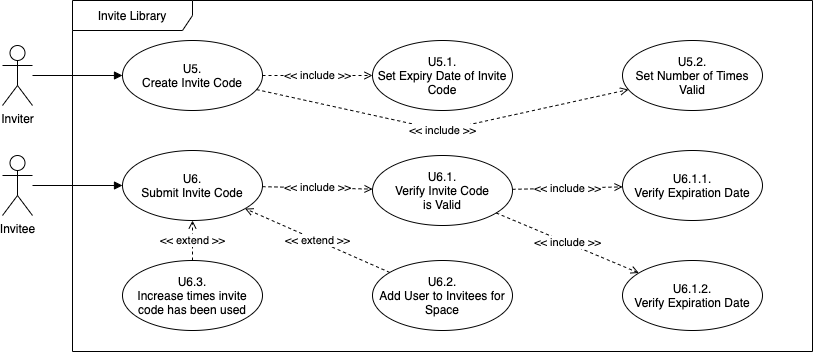
\includegraphics[width=1.0\textwidth]{documentation/software_requirements_specification/subsystems/invite_library_use_case.png}
  \caption{Invite Library Use Case Diagram}
  \label{fig:invite_library_use_case}
\end{figure}

\newpage

\subsection{Traceability Matrices}

\subsubsection{Subsystem traceability matrix}
The traceability matrix depicted in table \ref{tab:subsystem_traceability_matrix} below details how the main use cases of the Invite Only system, depicted in figure \ref{fig:invite_only_use_case} correspond to the functional requirements detailed in section \ref{Functional Requirements}.

\begin{table}[H]
\centering
\begin{tabular}{|l|c|c|c|c|c|c|}
\hline
        & U1. & U2. & U3. & U4. & U5. & U6. \\ \hline
R1.     & X   & X   & X   &     &     &     \\ \hline
R1.1.   & X   &     &     &     &     &     \\ \hline
R1.2.   &     & X   &     &     &     &     \\ \hline
R1.2.1  &     & X   &     &     &     &     \\ \hline
R1.2.2. &     & X   &     &     &     &     \\ \hline
R1.2.3. &     & X   &     &     &     &     \\ \hline
R1.2.4. &     & X   &     &     &     &     \\ \hline
R1.2.5. &     & X   &     &     &     &     \\ \hline
R1.2.6. &     & X   &     &     &     &     \\ \hline
R1.3.   &     &     & X   &     &     &     \\ \hline
R1.3.1. &     &     & X   &     &     &     \\ \hline
R1.3.2. &     &     & X   &     &     &     \\ \hline
R2.     & X   &     &     & X   &     &     \\ \hline
R2.1.   & X   &     &     &     &     &     \\ \hline
R2.2.   &     &     &     & X   &     &     \\ \hline
R3.     & X   &     &     &     & X   &     \\ \hline
R3.1.   & X   &     &     &     &     &     \\ \hline
R3.2.   &     &     &     &     & X   &     \\ \hline
R4.     &     &     &     &     &     &     \\ \hline
R4.1.   & X   &     &     &     &     & X   \\ \hline
R4.2.   & X   &     &     &     &     &     \\ \hline
R4.3.   &     &     &     &     &     & X   \\ \hline
R5.     & X   &     &     &     &     &     \\ \hline
\end{tabular}
\caption{Subsystem Traceability Matrix}
\label{tab:subsystem_traceability_matrix}
\end{table}

\newpage

\subsubsection{System Traceability Matrix}
The traceability matrix depicted in table \ref{tab:system_traceability_matrix} below details which of the subsystems described by the preceding use case diagrams will be involved when delivering each functional requirement.

\begin{table}[H]
\centering
\begin{tabular}{|l|c|c|c|c|}
\hline
        & User Library & Space Library & Access Library & Invite Library \\ \hline
R1.     & X            & X             & X              &                \\ \hline
R1.1.   & X            &               &                &                \\ \hline
R1.2.   &              & X             &                &                \\ \hline
R1.2.1  &              & X             &                &                \\ \hline
R1.2.2. &              & X             &                &                \\ \hline
R1.2.3. &              & X             &                &                \\ \hline
R1.2.4. &              & X             &                &                \\ \hline
R1.2.5. &              & X             &                &                \\ \hline
R1.2.6. &              & X             &                &                \\ \hline
R1.3.   &              &               & X              &                \\ \hline
R1.3.1. &              &               & X              &                \\ \hline
R1.3.2. &              &               & X              &                \\ \hline
R2.     & X            &               & X              &                \\ \hline
R2.1.   & X            &               &                &                \\ \hline
R2.2.   &              &               & X              &                \\ \hline
R3.     & X            &               &                & X              \\ \hline
R3.1.   & X            &               &                &                \\ \hline
R3.2.   &              &               &                & X              \\ \hline
R4.     & X            &               &                & X              \\ \hline
R4.1.   & X            &               &                &                \\ \hline
R4.2.   & X            &               &                &                \\ \hline
R4.3.   &              &               &                & X              \\ \hline
R5.     & X            &               &                &                \\ \hline
\end{tabular}
\caption{System Traceability Matrix}
\label{tab:system_traceability_matrix}
\end{table}

\newpage

\subsection{Actor-System Interaction models}

\subsubsection{User Library}

\begin{table}[H]
\centering
\begin{tabular}{|l|l|}
\hline
\multicolumn{2}{|c|}{\textbf{Precondition}}                                         \\ \hline
\multicolumn{2}{|l|}{\textit{none}}                                                 \\ \hline
\multicolumn{1}{|c|}{\textbf{Actor: User}} & \multicolumn{1}{c|}{\textbf{System: User Library}} \\ \hline
0. Open Application                             & 1. Display Authentication Options \\ \hline
2. Select Authentication Option & 3. Authenticate User              \\ \hline
\multicolumn{2}{|c|}{\textbf{Postcondition}}                                        \\ \hline
\multicolumn{2}{|l|}{\textit{User authenticated and session started}}               \\ \hline
\end{tabular}
\caption{User Authentication Interaction Model}
\label{tab:user_authentication_interaction}
\end{table}

\begin{table}[H]
\centering
\begin{tabular}{|l|l|}
\hline
\multicolumn{2}{|c|}{\textbf{Precondition}}                                                \\ \hline
\multicolumn{2}{|l|}{\textit{Identification document barcode is valid - throws invalid\_id}}    \\ \hline
\multicolumn{1}{|c|}{\textbf{Actor: User}} & \multicolumn{1}{c|}{\textbf{System: User Library}} \\ \hline
0. Add new document option & 1. Display scanner                      \\ \hline
2. Scan document barcode    & 3. Decode barcode and display details              \\ \hline
4. Confirm details                               & 5. Add document to user profile \\ \hline
\multicolumn{1}{|c|}{\textbf{Postcondition}}     &                                         \\ \hline
\multicolumn{2}{|l|}{\textit{Identification document details linked to user profile}}           \\ \hline
\end{tabular}
\caption{Link ID Document Interaction Model}
\label{tab:link_id_interaction}
\end{table}

\begin{table}[H]
\centering
\begin{tabular}{|l|l|}
\hline
\multicolumn{2}{|c|}{\textbf{Precondition}}                                       \\ \hline
\multicolumn{2}{|l|}{\textit{User is authenticated - throws user\_authentication\_error}}       \\ \hline
\multicolumn{1}{|c|}{\textbf{Actor: User}} & \multicolumn{1}{c|}{\textbf{System: User Library}} \\ \hline
0. Request deletion of Profile               & 1. Display confirmation message    \\ \hline
2. Confirm deletion                          & 3. Delete user profile from system \\ \hline
\multicolumn{1}{|c|}{\textbf{Postcondition}} &                                    \\ \hline
\multicolumn{2}{|l|}{\textit{All user details and associated data removed from system}}         \\ \hline
\end{tabular}
\caption{Delete User Interaction Model}
\label{tab:delete_user_interaction}
\end{table}

\subsubsection{Space Library}

\begin{table}[H]
\centering
\begin{tabular}{|l|l|}
\hline
\multicolumn{2}{|c|}{\textbf{Precondition}}                                           \\ \hline
\multicolumn{2}{|l|}{\textit{Required space details are available - throws validation\_error}} \\ \hline
\multicolumn{1}{|c|}{\textbf{Actor: Manager}} & \multicolumn{1}{c|}{\textbf{System: Space Library}} \\ \hline
0. Create new space option        & 1. Display space details form           \\ \hline
2. Submit name and access constraints & 3. Save space \\ \hline
\multicolumn{2}{|c|}{\textbf{Postcondition}}                                          \\ \hline
\multicolumn{2}{|l|}{\textit{New space has been saved}}                                        \\ \hline
\end{tabular}
\caption{Create Space Interaction Model}
\label{tab:create_space_interaction}
\end{table}

\begin{table}[H]
\centering
\begin{tabular}{|l|l|}
\hline
\multicolumn{2}{|c|}{\textbf{Precondition}}                             \\ \hline
\multicolumn{2}{|l|}{\textit{User has rights to delete space - throws invalid\_permissions}}        \\ \hline
\multicolumn{1}{|c|}{\textbf{Actor: Manager}} & \multicolumn{1}{c|}{\textbf{System: Space Library}} \\ \hline
0. Select option to delete space   & 1. Display confirmation message    \\ \hline
2. Confirm deletion                & 3. Remove space and related data   \\ \hline
\multicolumn{2}{|c|}{\textbf{Postcondition}}                            \\ \hline
\multicolumn{2}{|l|}{\textit{Space details have been entirely removed}} \\ \hline
\end{tabular}
\caption{Delete Space Interaction Model}
\label{tab:delete_space_interaction}
\end{table}

\subsubsection{Access Library}

\begin{table}[H]
\centering
\begin{tabular}{|l|l|}
\hline
\multicolumn{2}{|c|}{\textbf{Precondition}}                            \\ \hline
\multicolumn{2}{|l|}{\textit{User has rights to view access history - throws invalid\_permissions}}  \\ \hline
\multicolumn{1}{|c|}{\textbf{Actor: Manager}} & \multicolumn{1}{c|}{\textbf{System: Access Library}} \\ \hline
0. Open space                    & 1. Display access history for space \\ \hline
2. Add filters to access history & 3. Filter access history            \\ \hline
\multicolumn{2}{|c|}{\textbf{Postcondition}}                           \\ \hline
\multicolumn{2}{|l|}{\textit{Access history is displayed according to filters}}                      \\ \hline
\end{tabular}
\caption{View Access Metrics Interaction Model}
\label{tab:access_metrics_interaction}
\end{table}

\begin{table}[H]
\centering
\begin{tabular}{|l|l|}
\hline
\multicolumn{2}{|c|}{\textbf{Precondition}}                                              \\ \hline
\multicolumn{2}{|l|}{\textit{Scanned identity document is valid - throws invalid\_id}}   \\ \hline
\multicolumn{1}{|c|}{\textbf{Actor: Guard}} & \multicolumn{1}{c|}{\textbf{System: Access Library}} \\ \hline
0. Request to grant access          & 1. Display scanner                                 \\ \hline
2. Scan identification document     & 3. Validate access    \\ \hline
\multicolumn{2}{|c|}{\textbf{Postcondition}}                                             \\ \hline
\multicolumn{2}{|l|}{\textit{Message informing guard to allow/deny access is displayed}} \\ \hline
\end{tabular}
\caption{Allow/Deny Access Interaction Model}
\label{tab:access_interaction}
\end{table}

\subsubsection{Invite Library}

\begin{table}[H]
\centering
\begin{tabular}{|l|l|}
\hline
\multicolumn{2}{|c|}{\textbf{Precondition}}                    \\ \hline
\multicolumn{2}{|l|}{\textit{User is invitee for space - throws invalid\_permissions}}             \\ \hline
\multicolumn{1}{|c|}{\textbf{Actor: Inviter}} & \multicolumn{1}{c|}{\textbf{System: Invite Library}} \\ \hline
0. Request new invite code        & 1. Generate and display invite code            \\ \hline
2. Select option to share       & 3. Share invite code    \\ \hline
\multicolumn{2}{|c|}{\textbf{Postcondition}}                   \\ \hline
\multicolumn{2}{|l|}{\textit{Invite code is saved and shared}} \\ \hline
\end{tabular}
\caption{Create Invite Code Interaction Model}
\label{tab:create_invite_interaction}
\end{table}

\begin{table}[H]
\centering
\begin{tabular}{|l|l|}
\hline
\multicolumn{2}{|c|}{\textbf{Precondition}}                                    \\ \hline
\multicolumn{2}{|l|}{\textit{Invite code is valid - throws invalid\_code}}     \\ \hline
\multicolumn{1}{|c|}{\textbf{Actor: Invitee}} & \multicolumn{1}{c|}{\textbf{System: Invite Library}} \\ \hline
0. Submit invite code       & 1. Display linked space \\ \hline
2. Confirm space is correct & 3. Add user as invitee to space                  \\ \hline
\multicolumn{2}{|c|}{\textbf{Postcondition}}                                   \\ \hline
\multicolumn{2}{|l|}{\textit{User has been added as invitee and is allowed access to a space}}       \\ \hline
\end{tabular}
\caption{Submit Invite Code Interaction Model}
\label{tab:subkit_invite_interaction}
\end{table}